\subsection{Research Context}

\almarginpar{I cannot fit it below, so I include it here: Are the Table 1 elements in any way related to the experimental work? How? Is the number of experiments determined by the cases included in the table? Any relation with Figure 9?}
As explained in the previous section (Section \ref{Literature Review section}), the VQA approach to circuit design for QNN construction overcomes many constraints of the NISQ devices. It allows the construction of trainable circuits, which support the development of practical applications in optimisation and machine learning.
However, we have observed the existence of barren plateaus, causing the variance of the cost function gradient to vanish exponentially with the number of qubits.
We have thus investigated three methods to mitigate this phenomenon, i.e. by using a local cost function with shallow circuits, by relying on the identity block and by utilising layerwise learning \cite{cerezoCostFunctionDependent2021, liuParameterInitializationMethod2021, skolikLayerwiseLearningQuantum2021}.

In the following sections, we will answer the study research question (see Section \ref{Problem Section}) by conducting a series of experiments such that different methods are applied to the same objects. 
This process is known as \emph{technology-oriented empirical research} \cite{wohlinExperimentationSoftwareEngineering2012}.

We summarise the adopted research process in Figure \ref{Research Activities Figure}.
Our main objects and the different technical treatments for the experiment are discussed in section \ref{Objects section}, the two phases of the experiment in section \ref{Research Activities section}, and finally the confirmation of results from the experiment in section \ref{Data Collecting Section}.
\almarginpar{You cannot just dump the figure with the research process, you need to explain what is in it, i.e. Figure 9 and the details of its three phases as related to sections 3.1.2 (where is it in the figure?), 3.1.3 (first and second phase), and what happened to the third? You still need to describe it}

\begin{figure}
    \centering
    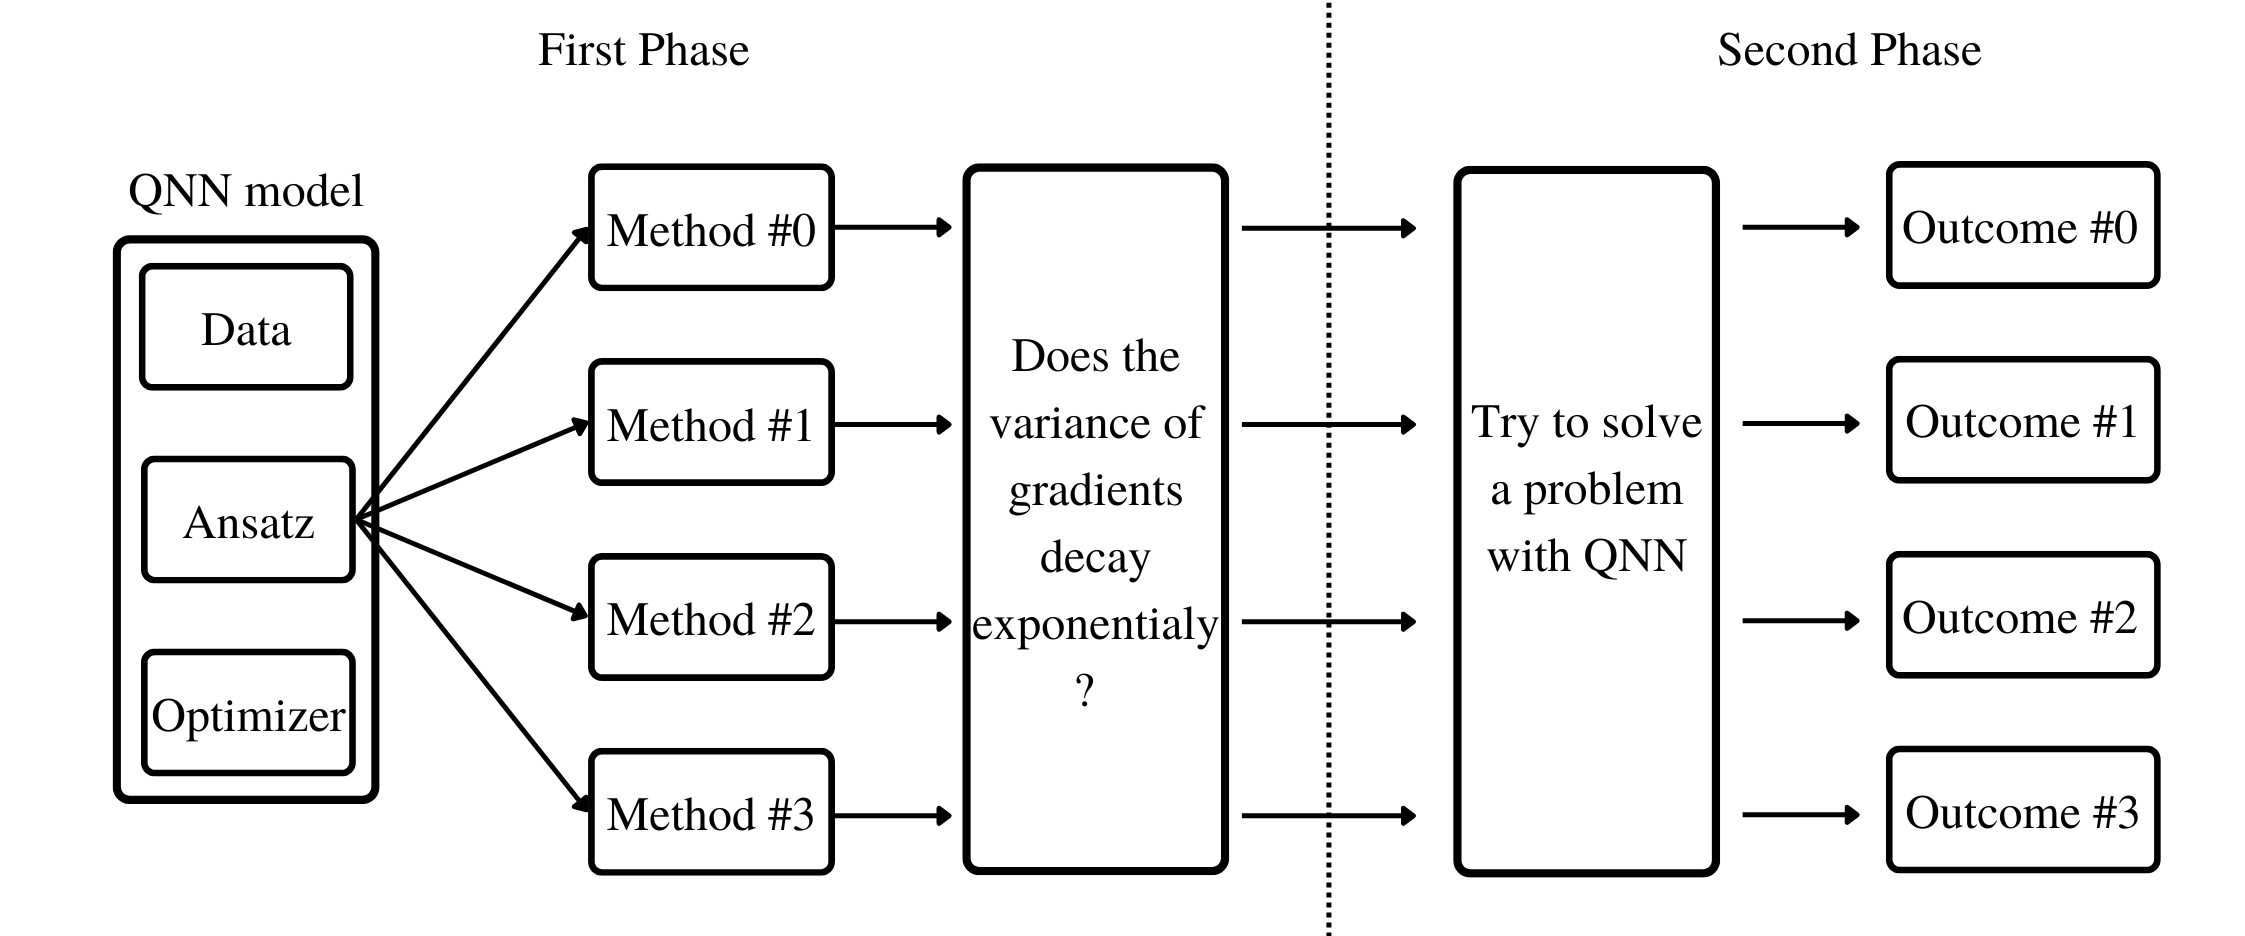
\includegraphics[width=\textwidth]{./ResearchDesign/Appendices/ExperimentDiagram.png}
    \caption{
        The adopted research process.
    }
    \label{Research Activities Figure}
\end{figure}
